\documentclass[12pt,letterpaper,english,bibliography=totocnumbered, abstract=on]{scrartcl}

\usepackage{indentfirst}
\usepackage[titletoc]{appendix}
\usepackage[T1]{fontenc}
\usepackage[latin9]{inputenc}
\usepackage{color}
\usepackage{babel}
\usepackage{verbatim}
\usepackage[unicode=true,pdfusetitle,
bookmarks=true,bookmarksnumbered=false,bookmarksopen=false,
breaklinks=true,pdfborder={0 0 0},pdfborderstyle={},backref=false,colorlinks=true]
{hyperref}
\hypersetup{linkcolor=blue,citecolor=blue,urlcolor=blue}

\usepackage{booktabs}
\usepackage{multirow}
\usepackage{adjustbox}
\usepackage{threeparttable}
\usepackage[table]{xcolor}
\usepackage{csquotes}
\usepackage{soul} % for hiliting text: \hl

\usepackage[backend=biber, style=authoryear, maxbibnames=99, dashed=false]{biblatex}
\setlength\bibitemsep{2\itemsep}
\addbibresource{CRB.bib}

\usepackage{pdfpages}
\usepackage{float} % Allows use of H to place floats

\usepackage{pgfgantt}

\usepackage{framed}

\usepackage{datetime2}

% Prevent page breaks within paragraphs
% https://tex.stackexchange.com/questions/21983/how-to-avoid-page-breaks-inside-paragraphs
\widowpenalties 1 10000

\begin{document}

%\titlehead{Titlehead}

\title{Notes for Background, Methods, and Results Sections of the CRB Trap Improvement Article}

\author{Aubrey Moore}

\date{\DTMnow}


\maketitle

\tableofcontents

\footnote{The most recent version of this document can be downloaded from\\
\url{https://github.com/aubreymoore/CRB-trap-improvement/blob/master/results.pdf}.}

\pagebreak

For computational details see the Jupyter notebook at:\\
\url{https://github.com/aubreymoore/CRB-trap-improvement/blob/master/xtraps.ipynb}

\section{Background}

\subsection{Depleted Lures}

In the island-wide trapping program pheromone traps baited with ChemTica oryctalure bubble packs were visited about every 2 weeks. Depleted lures, those with no liquid visible in the bubble pack,  were replaced and this was recorded in the trapping database. Traps with depleted lures caught significantly more beetles than those with undepleted lures (0.220 vs. 0.092 beetles per trap-visit; $P<0.001$ [Welch Two Sample t-test]) (For details see \cite{moore_research_2012}).

\section{Methods}

\subsection{Pheromone Lures}

We used Oryctalure pheromone dispensers manufactured by ChemTica. These lures are bubble packs which use a plastic
membrane to regulate the release rate of the CRB aggregation pheromone (ethyl 4-methyloctenate).
In this experiment, we weighed lures before deployment and after pick up so that we could measure
field release rates. Preliminary work showed that rain water entered Oryctalures making it impos-
sible to accurately measure release rates. To solve this problem, we heat-sealed each Oryctalure
into a thin polyethylene bag, reducing the release rate by about 10\%. 

We made reduced-release
rate pheromone dispensers by placing 200 microlitres of liquid removed from an Oryctalure into a 2 ml Eppendorf
centrifuge tube with a 2 mm (5/64 inch) hole drilled in its top. The centrifuge tube was then placed
in a pottle which acted as a rain and wind shield (\ref{fig:reduced-release-rate-device}).

For details see \cite{moore_technical_2013}.

\begin{figure}[h]
	\centering
	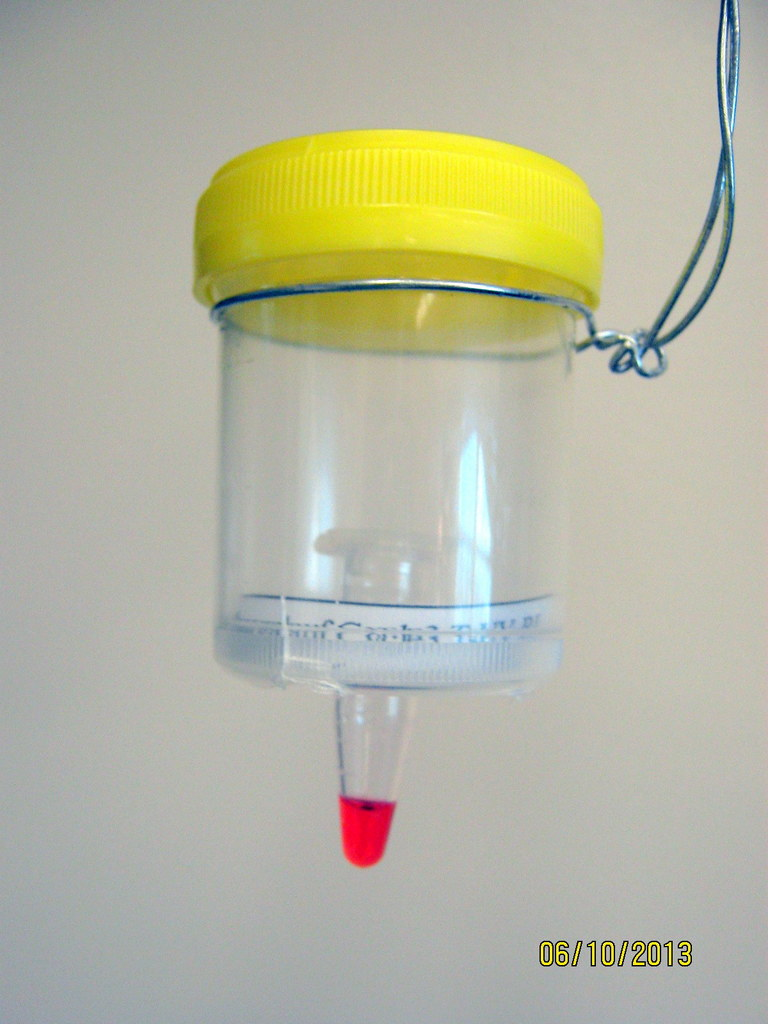
\includegraphics[width=0.5\linewidth]{images/reduced-release-rate-device}
	\caption{
		Reduced release rate pheromone dispenser.
		\hl{I will replace this image with a better one which shows holes in bottom of pottle.}}
	\label{fig:reduced-release-rate-device}
\end{figure}


\clearpage

\subsection{Ultraviolet Light Emitting Diodes}

Solar charged, ultraviolet light emitting diodes were made from garden path lights by replacing the standard white LED with an ultraviolet LED with a dominant wavelength of 400-405 nm and a luminous intensity of 80-120 mcd. The lens of the LED UVLED was scuffed with sandpaper to make it diffuse and omnidirectional. Further specifications and construction details are in \cite{moore_solar_2013}.

Relative attractiveness of the white diode installed in garden path lights and the UVLED custom replacement was measured in a large field cage test. Two barrel traps were placed side by side and an orytalure was placed between them. One trap was fitted with white LED and the other was fitted with a UV LED.  The trap with the white LED caught 15 beetles and the trap with the UV LED caught 100 beetles. The difference in trap catch was highly significant (binomial test; $P<0.001$). Details can be found in \cite{moore_relative_2014}.

\clearpage

\section{Results}

\subsection{Trap Catch Summary}

\begin{table}[h]
	\caption{Capture summary by trap type.}
	\tiny
	\centering
	\begin{tabular}{@{}llccccc@{}}
		\toprule
		Trap type & \multicolumn{1}{c}{Description} & \multicolumn{3}{c}{Beetles trapped} & \begin{tabular}[c]{@{}c@{}}Proportion of\\traps which caught\\one or more beetles\\during 2 week\\trapping periods\end{tabular} & \begin{tabular}[c]{@{}c@{}}Beetles caught\\per trap-day\\(mean $\pm$ SEM)\end{tabular} \\ \midrule
		&  & Male & Female & Total &  &  \\ \cmidrule(lr){3-5}
		T & \begin{tabular}[c]{@{}l@{}}Trap with no lure\\ and no UVLED\end{tabular} & 0 & 0 & 0 & 0/36 & 0.000 $\pm$ 0.000 \\
		T-UV & \begin{tabular}[c]{@{}l@{}}Trap with no lure\\ and UVLED\end{tabular} & 0 & 2 & 2 & 2/36 & 0.003 $\pm$ 0.002 \\
		T-RL & \begin{tabular}[c]{@{}l@{}}Trap with reduced release\\ rate lure\end{tabular} & 9 & 4 & 13 & 7/36 & 0.027 $\pm$ 0.012 \\
		T-SL & \begin{tabular}[c]{@{}l@{}}Trap with standard release\\ rate lure\end{tabular} & 11 & 9 & 20 & 10/36 & 0.039 $\pm$ 0.014 \\
		T-UV-RL & \begin{tabular}[c]{@{}l@{}}Trap with reduced release\\ rate lure and UVLED\end{tabular} & 18 & 20 & 38 & 12/36 & 0.073 $\pm$ 0.025 \\
		T-UV-SL & \begin{tabular}[c]{@{}l@{}}Trap with standard release\\  rate lure and UVLED\end{tabular} & 30 & 24 & 54 & 15/36 & 0.109 $\pm$ 0.031 \\ \bottomrule
	\end{tabular}
\end{table}

\hl{
	MATT: Can we put letters after the means to signify significant differences? Not sure which multiple comparison test is appropriate for our data. If you are willing to take on this challenge, the raw data are available at:}\\
\footnotesize{\url{https://github.com/aubreymoore/CRB-trap-improvement/blob/master/trapType-captureRate.csv}}


\begin{figure}[h]
\centering
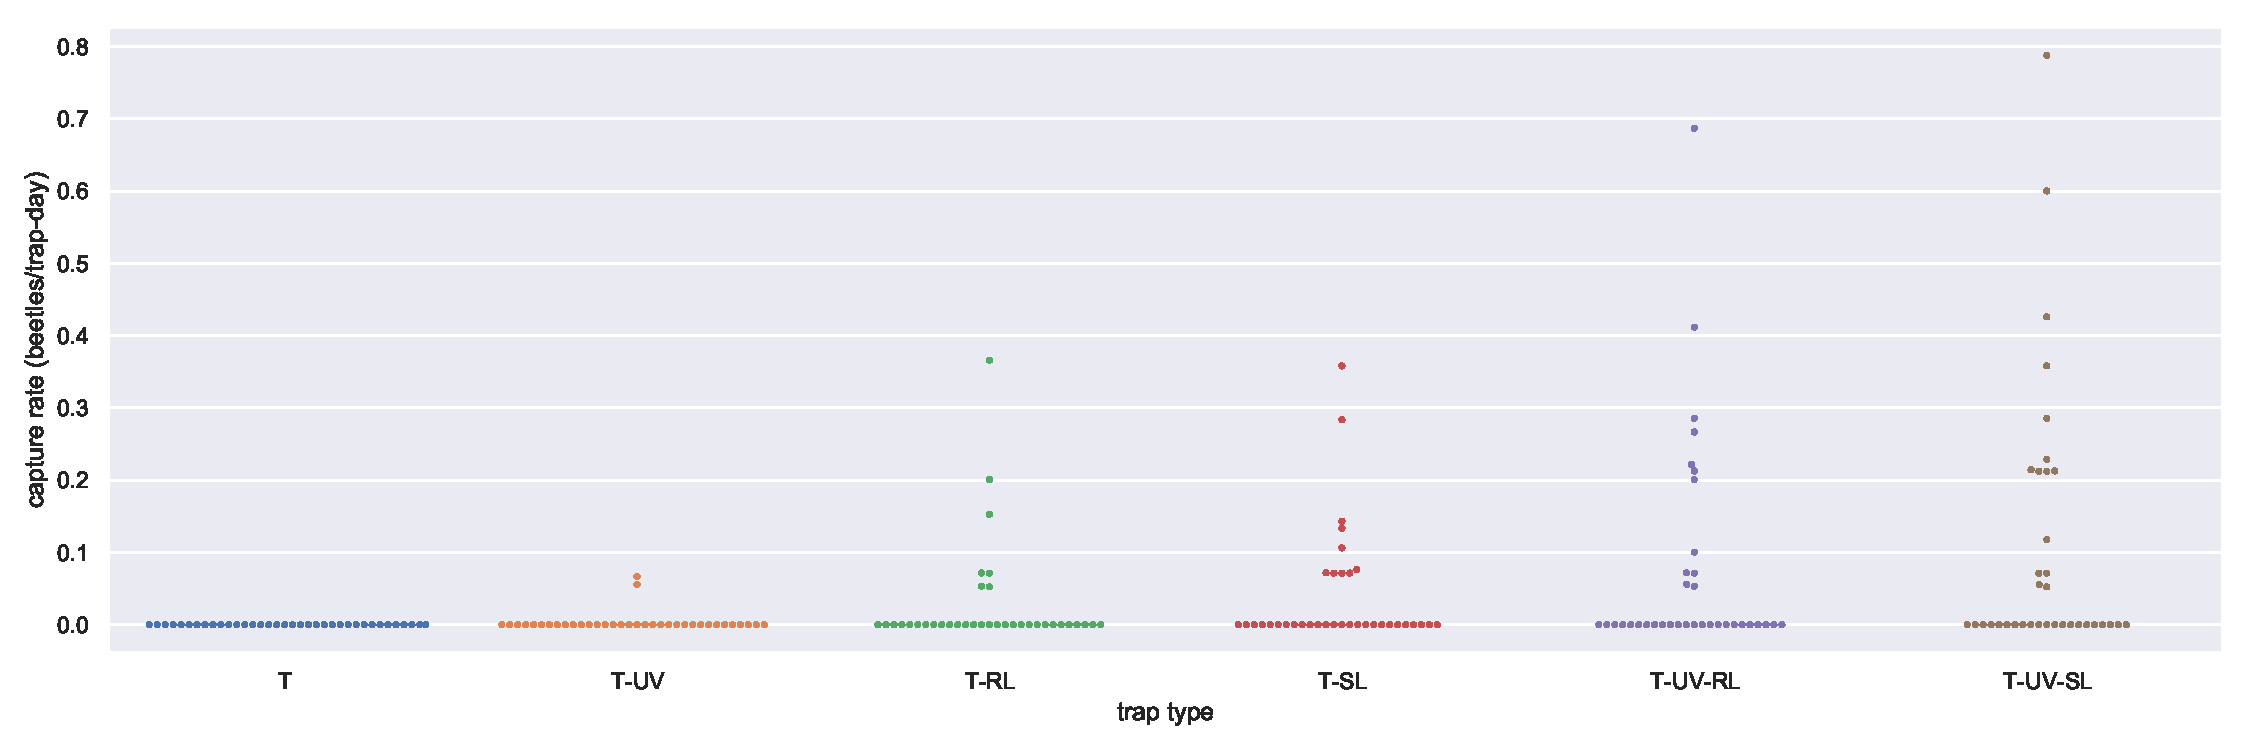
\includegraphics[width=1\linewidth]{images/trapcatch-swarmplot}
\caption{Capture rate by trap type. \hl{MATT: IMHO, this is the best way to display our data, see the Jupyter notebook for a couple of alternatives.}}
\label{fig:trapcatch-swarmplot}
\end{figure}

\begin{itemize}
	\item For all trap types, sex ratio was not significantly different from 50:50 (binomial test).
	\item For all trap types, most traps contained no beetles at the end of each trap cycle, nominally 2 weeks.
\end{itemize}


\newpage

\subsection{Capture Rate as a Function of Pheromone Release Rate}

\begin{figure}[h]
\centering
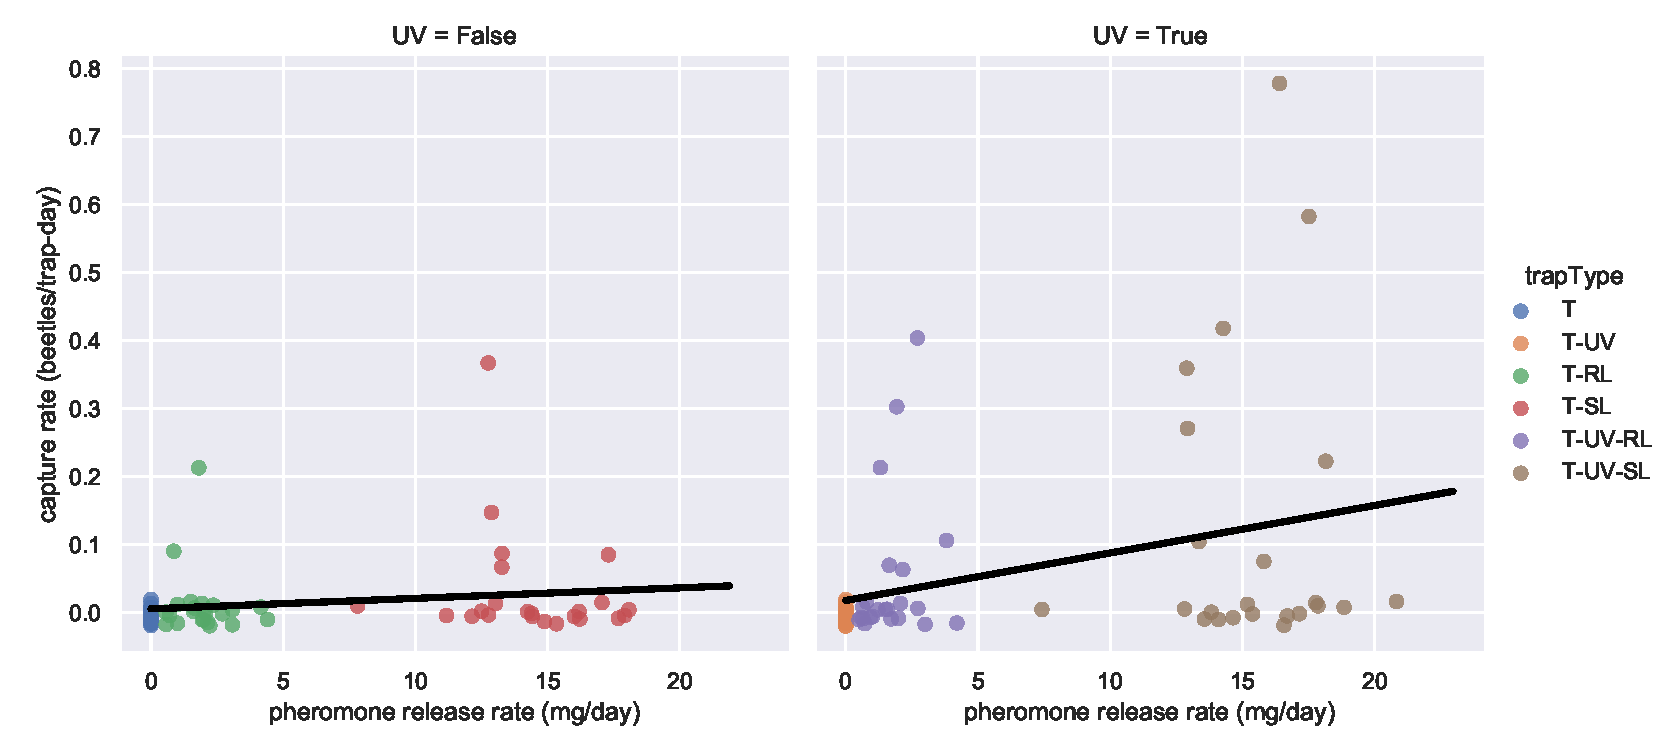
\includegraphics[width=1\linewidth]{images/trapcatch-lmplot}
\caption{
	Capture rate as a function of pheromone release rate for traps with and without ultraviolet light emitting diodes.
	Lines are ordinary least-squares fits.	
	The equation for traps without UVLEDs is $y = 0.0059 + 0.0015x$; slope is not significantly different from zero ($P=0.118$).
	The equation for traps with UVLEDs is $y = 0.0182 + 0.0070x$; slope is significantly different from zero ($P=0.005$).
	}
\label{fig:trapcatch-lmplot}
\end{figure}

\printbibliography	

\end{document}
